%<*mtag1>
\begin{figure}[H]
\centering
\captionsetup{width=.8\linewidth}
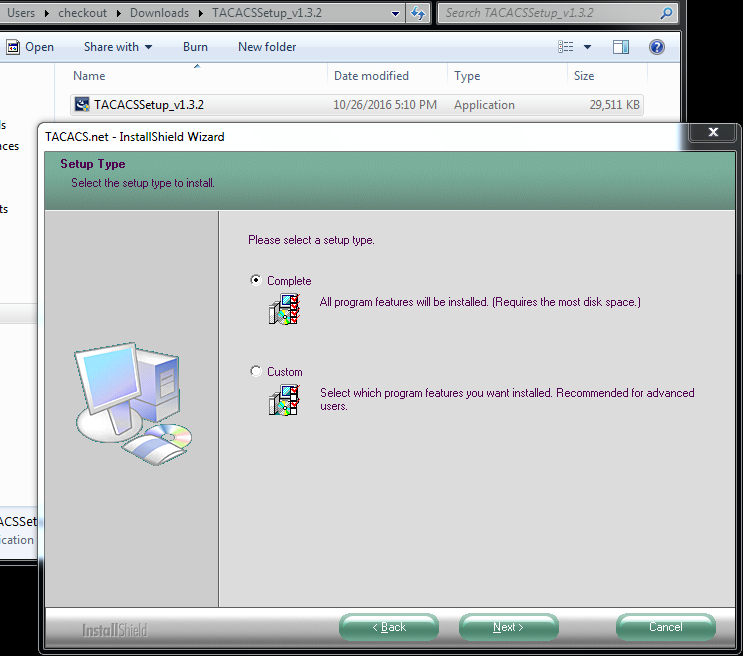
\includegraphics[scale=0.5]{img/1_tacacssetup.PNG}
\caption{Shows the installation wizard of TACACS+ server on Windows 7 vm}
\label{fig:}
\centering
\end{figure}
%</mtag1>

%<*mtag2>
\begin{figure}[H]
\centering
\captionsetup{width=.8\linewidth}
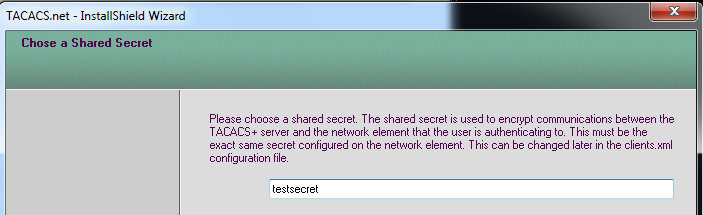
\includegraphics[scale=0.5]{img/2_testsecret.PNG}
\caption{Setting of the secret encryption key "testsecret" in the wizard.}
\label{fig:}
\centering
\end{figure}
%</mtag2>

%<*mtag3>
\begin{figure}[H]
\centering
\captionsetup{width=.8\linewidth}
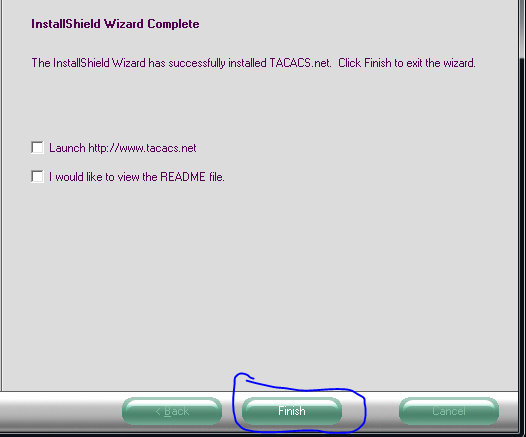
\includegraphics[scale=0.5]{img/3_installed.PNG}
\caption{Finishing the installation.}
\label{fig:}
\centering
\end{figure}
%</mtag3>

%<*mtag4>
\begin{figure}[H]
\centering
\captionsetup{width=.8\linewidth}
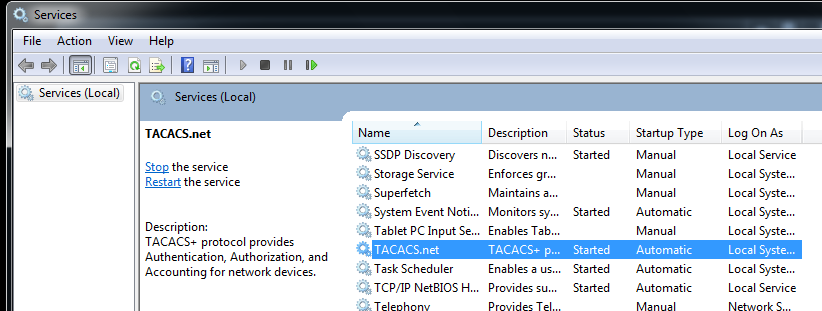
\includegraphics[scale=0.6]{img/4_services.PNG}
\caption{Checking that the server is up and running through the control panel.}
\label{fig:services}
\centering
\end{figure}
%</mtag4>

%<*mtag5>
\begin{figure}[H]
\centering
\captionsetup{width=.8\linewidth}
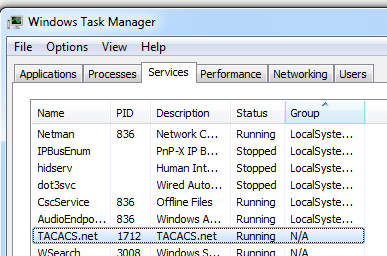
\includegraphics[scale=0.7]{img/5_taskmanager.PNG}
\caption{Checking the task manager to see that the TACACS.net server is running.}
\label{fig:tasks}
\centering
\end{figure}
%</mtag5>

%<*mtag6>
\begin{figure}[H]
\centering
\captionsetup{width=.8\linewidth}
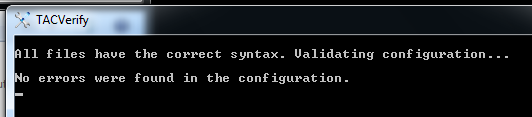
\includegraphics[scale=0.7]{img/6_tacverify.PNG}
\caption{Shows the running of tacverify, to see if the default configurations were in working order.}
\label{fig:}
\centering
\end{figure}
%</mtag6>

%<*mtag7>
\begin{figure}[H]
\centering
\captionsetup{width=.8\linewidth}
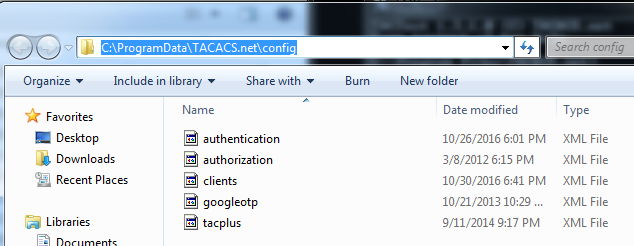
\includegraphics[scale=0.5]{img/7_config.PNG}
\caption{}
\label{fig:}
\centering
\end{figure}
%</mtag7>

%<*mtag8>
\begin{figure}[H]
\centering
\captionsetup{width=.8\linewidth}
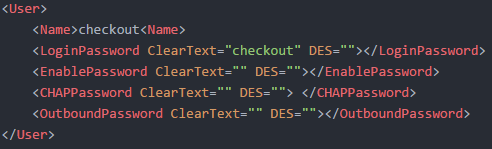
\includegraphics[scale=0.5]{img/7_testuser.PNG}
\caption{}
\label{fig:}
\centering
\end{figure}
%</mtag8>

%<*mtag9>
\begin{figure}[H]
\centering
\captionsetup{width=.8\linewidth}
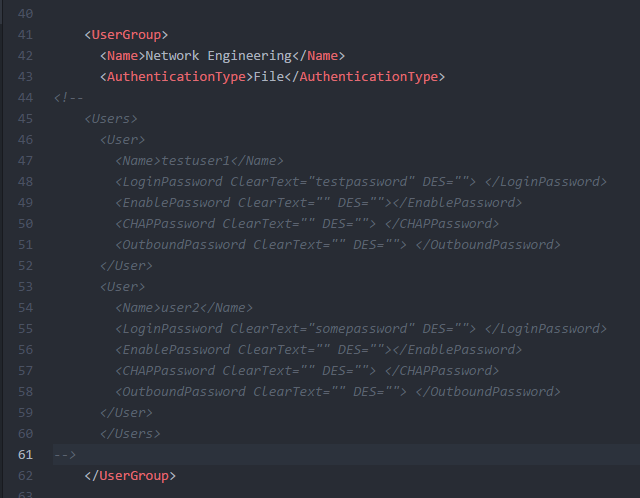
\includegraphics[scale=0.5]{img/8_commentusers.PNG}
\caption{}
\label{fig:}
\centering
\end{figure}
%</mtag9>

%<*mtag10>
\begin{figure}[H]
\centering
\captionsetup{width=.8\linewidth}
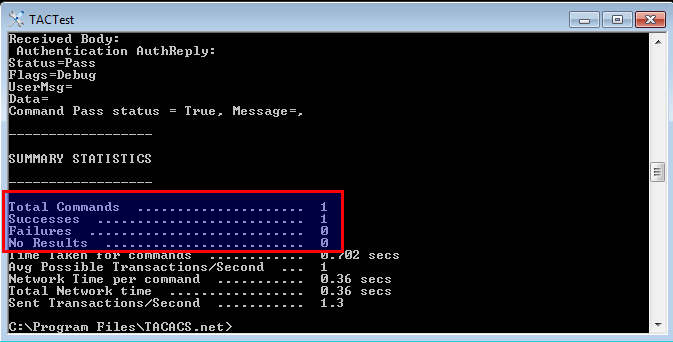
\includegraphics[scale=0.5]{img/tactestsucceed.png}
\caption{Proof that the tactest tool built into the TACACS.net software succeeded  with the user we created.}
\label{fig:tactestsucceed}
\centering
\end{figure}
%</mtag10>

%<*mtag10.1>
\begin{figure}[H]
\centering
\captionsetup{width=.8\linewidth}
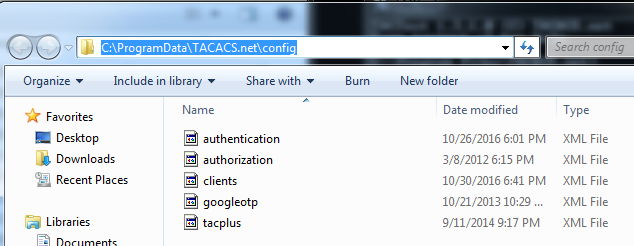
\includegraphics[scale=0.5]{img/7_config.PNG}
\caption{Shows the different configuartion files available to us in TACACS.net}
\label{fig:7config}
\centering
\end{figure}
%</mtag10.1>

%<*mtag10.2>
\begin{figure}[H]
\centering
\captionsetup{width=.8\linewidth}
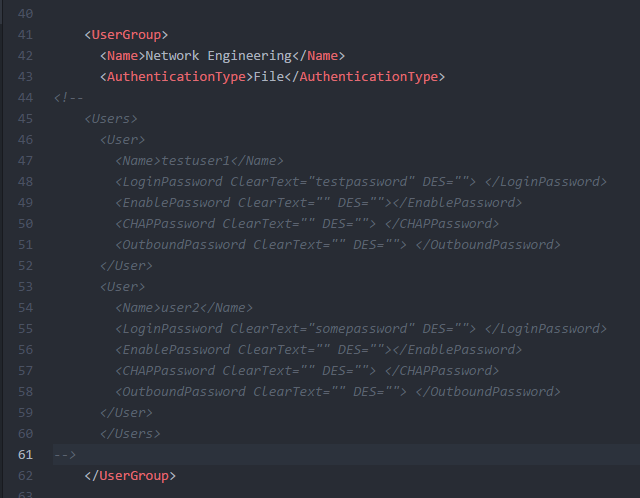
\includegraphics[scale=0.5]{img/8_commentusers.PNG}
\caption{}
\label{fig:8users}
\centering
\end{figure}
%</mtag10.2>

%<*mtag10.3>
\begin{figure}[H]
\centering
\captionsetup{width=.8\linewidth}
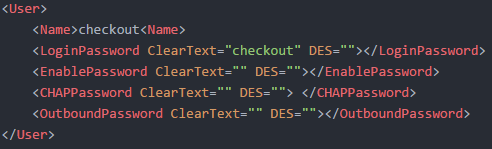
\includegraphics[scale=0.5]{img/7_testuser.PNG}
\caption{Shows the part of TACACS.net that automatically populated a user "checkout", our local account credentials.}
\label{fig:localuser}
\centering
\end{figure}
%</mtag10.3>



%<*mtag11>
\begin{figure}[H]
\centering
\captionsetup{width=.8\linewidth}
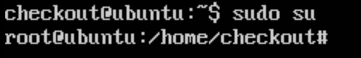
\includegraphics[scale=0.5]{img/Ex1_1.png}
\caption{Elevation to root}
\label{fig:}
\centering
\end{figure}
%</mtag11>

%<*mtag12>
\begin{figure}[H]
\centering
\captionsetup{width=.8\linewidth}
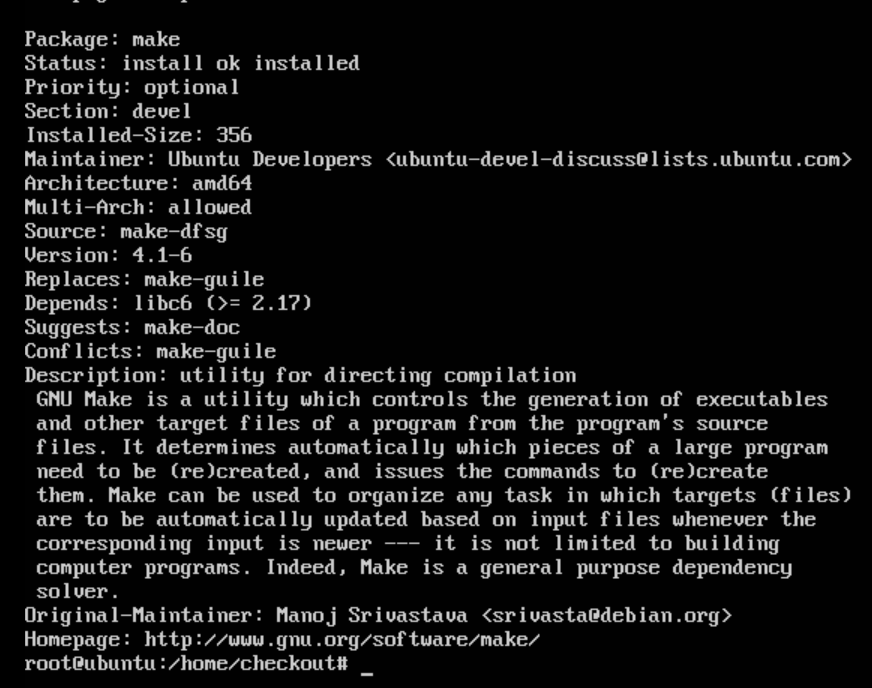
\includegraphics[scale=0.5]{img/Ex1_2.png}
\caption{dpkg output}
\label{fig:}
\centering
\end{figure}
%</mtag12>

%<*mtag13>
\begin{figure}[H]
\centering
\captionsetup{width=.8\linewidth}
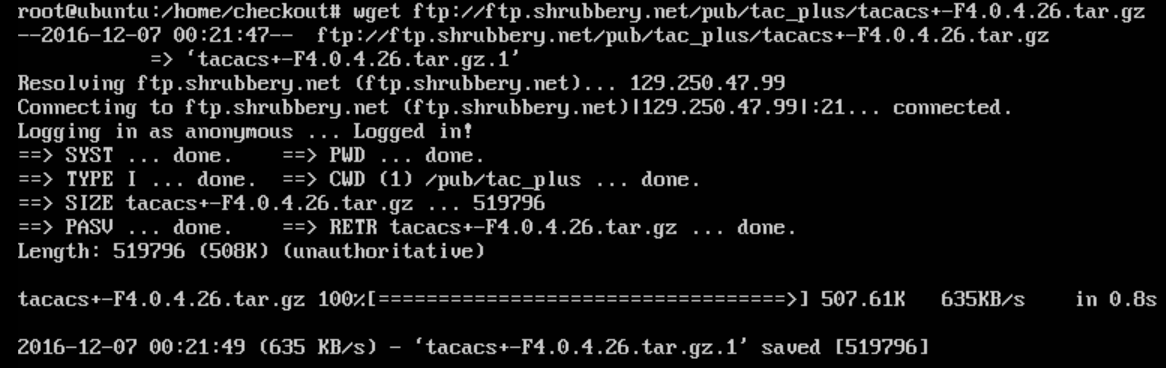
\includegraphics[scale=0.4]{img/Ex1_3.png}
\caption{Downloading tacacs}
\label{fig:}
\centering
\end{figure}
%</mtag13>

%<*mtag14>
\begin{figure}[H]
\centering
\captionsetup{width=.8\linewidth}
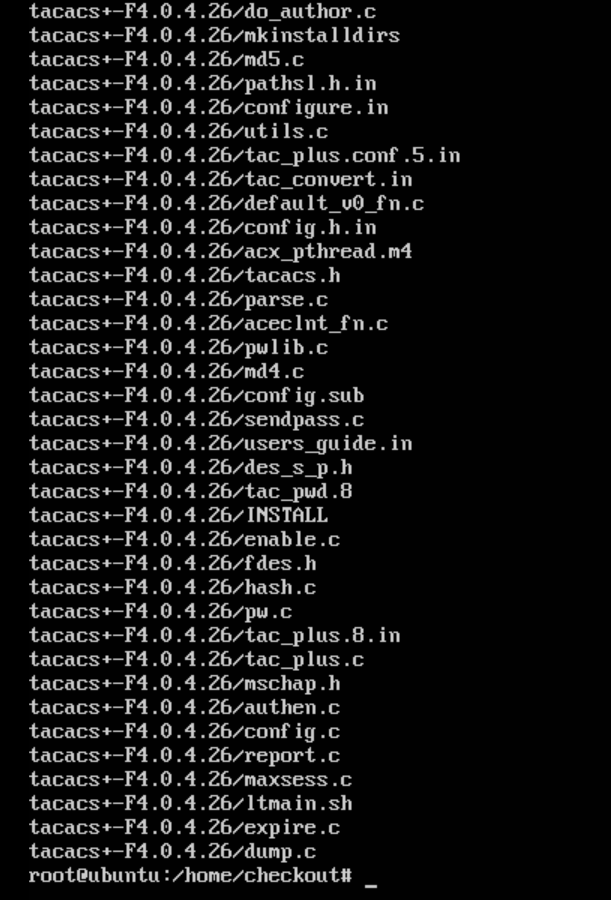
\includegraphics[scale=0.5]{img/Ex1_4.png}
\caption{Decompression of the downloaded file}
\label{fig:}
\centering
\end{figure}
%</mtag14>

%<*mtag15>
\begin{figure}[H]
\centering
\captionsetup{width=.8\linewidth}
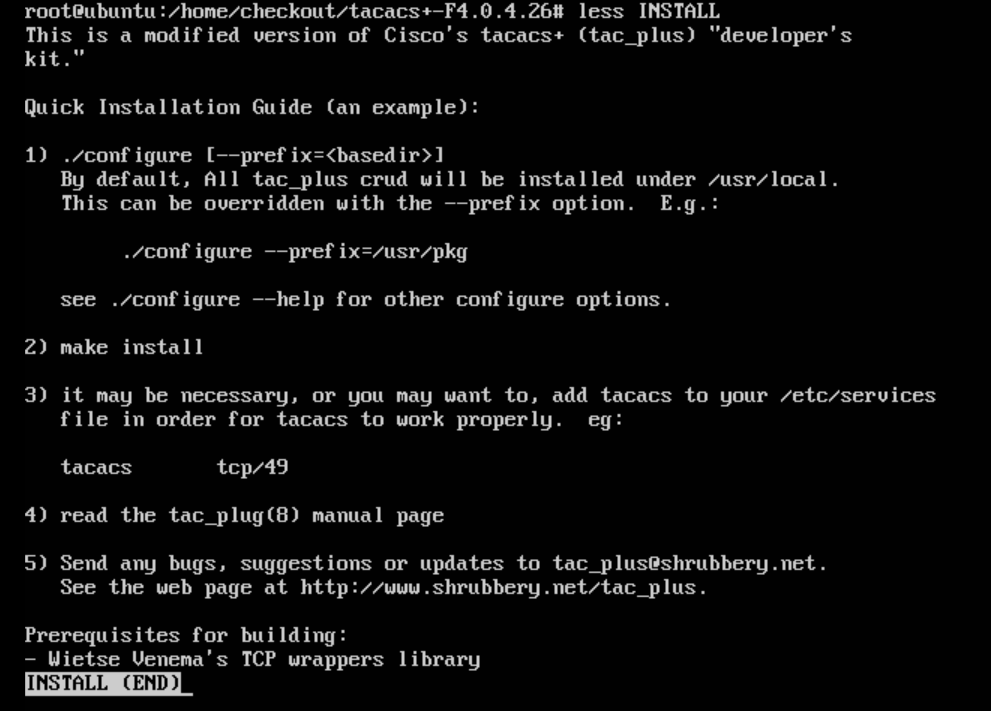
\includegraphics[scale=0.4]{img/Ex1_5.png}
\caption{Installation instructions}
\label{fig:}
\centering
\end{figure}
%</mtag15>

%<*mtag16>
\begin{figure}[H]
\centering
\captionsetup{width=.8\linewidth}
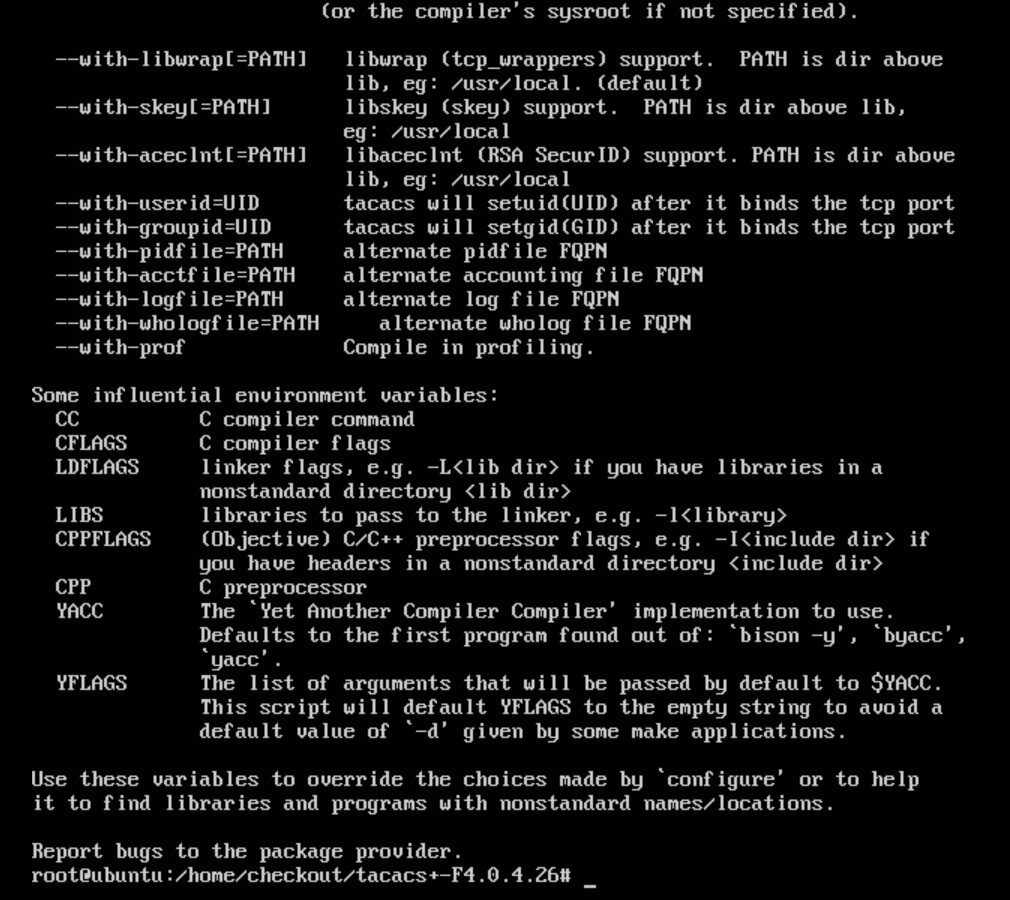
\includegraphics[scale=0.4]{img/Ex1_6.png}
\caption{config help}
\label{fig:}
\centering
\end{figure}
%</mtag16>

%<*mtag17>
\begin{figure}[H]
\centering
\captionsetup{width=.8\linewidth}
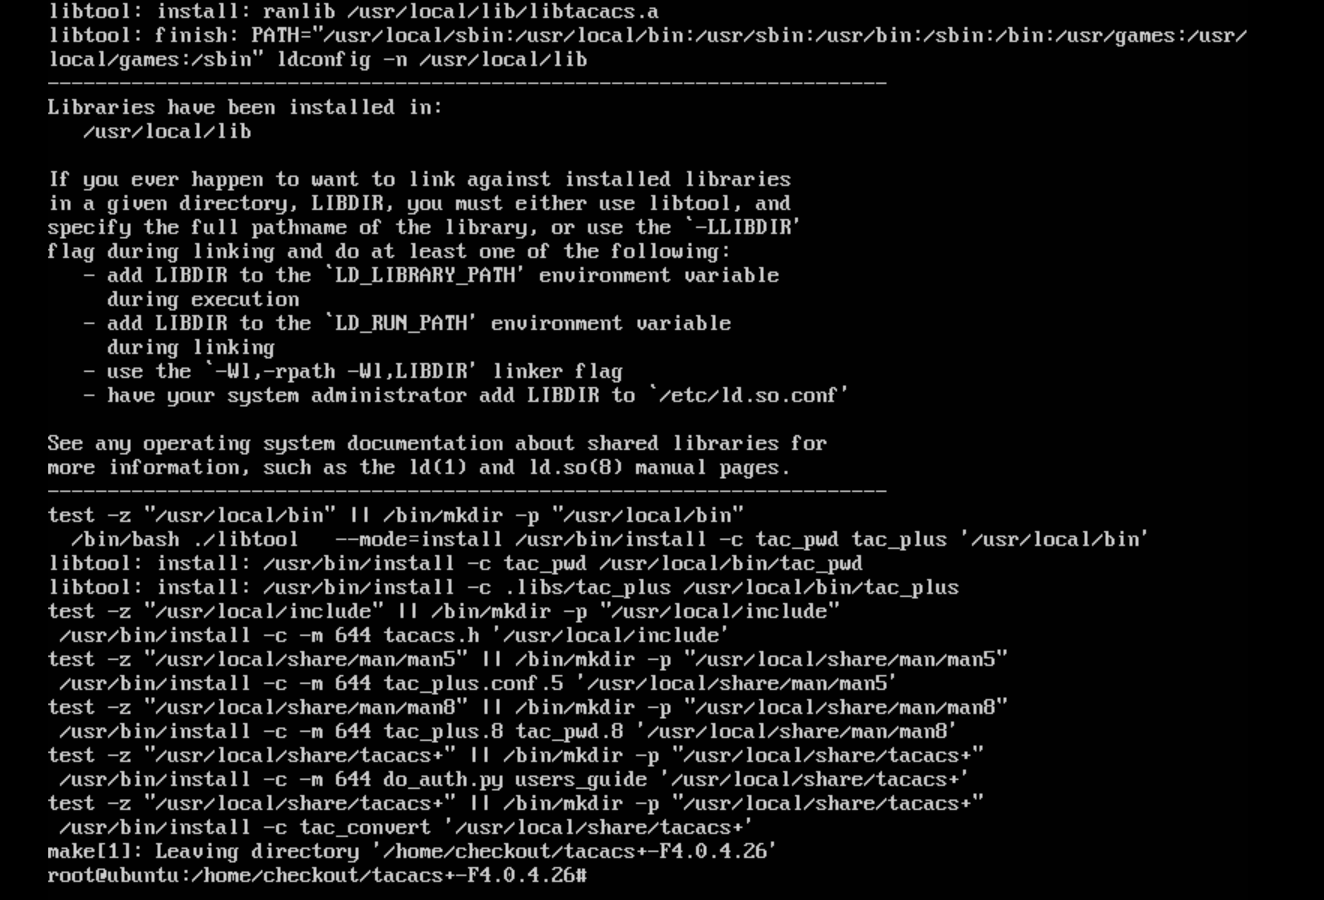
\includegraphics[scale=0.4]{img/Ex1_7.png}
\caption{Running the installation}
\label{fig:}
\centering
\end{figure}
%</mtag17>

%<*mtag18>
\begin{figure}[H]
\centering
\captionsetup{width=.8\linewidth}
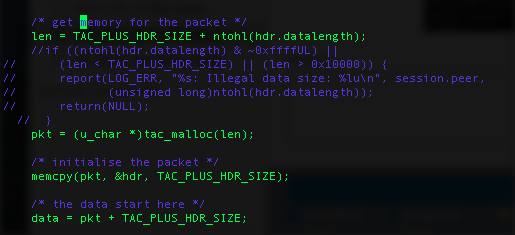
\includegraphics[scale=0.5]{img/tacacs_commented_out.png}
\caption{Code commented out}
\label{fig:}
\centering
\end{figure}
%</mtag18>

%<*mtag19>
\begin{figure}[H]
\centering
\captionsetup{width=.8\linewidth}
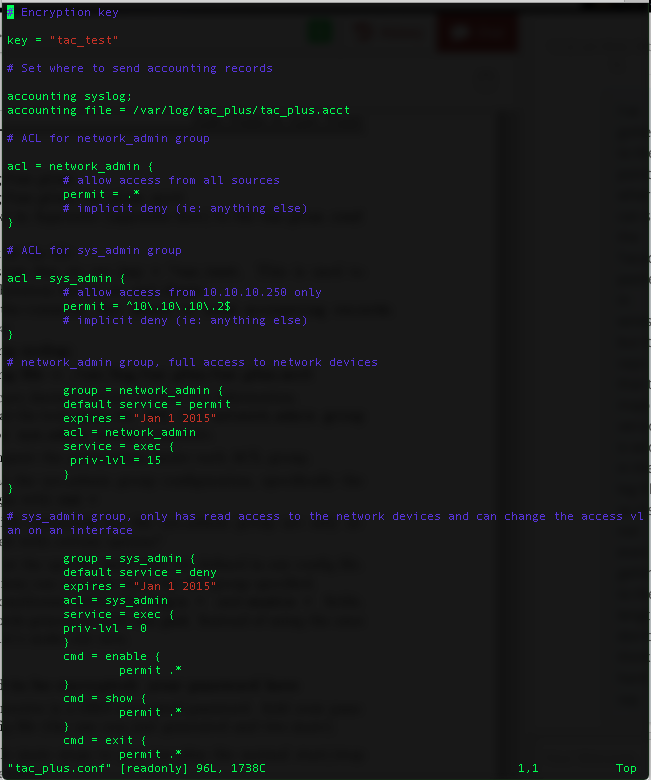
\includegraphics[scale=0.5]{img/tac_plus_conf.png}
\caption{Tacacs+ Config File}
\label{fig:}
\centering
\end{figure}
%</mtag19>

%<*mtag20>
\begin{figure}[H]
\centering
\captionsetup{width=.8\linewidth}
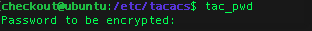
\includegraphics[scale=0.5]{img/tac_pwd.png}
\caption{Password Generation}
\label{fig:}
\centering
\end{figure}
%</mtag20>

%<*mtag21>
\begin{figure}[H]
\centering
\captionsetup{width=.8\linewidth}
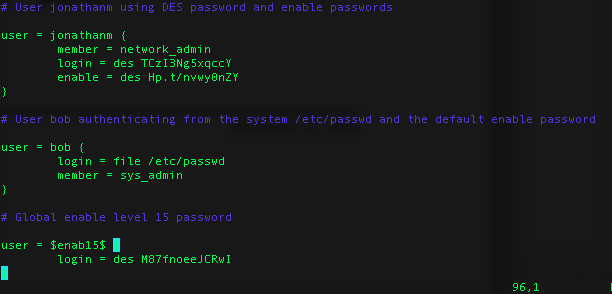
\includegraphics[scale=0.5]{img/conf_pass.png}
\caption{Passwords Added to the config file}
\label{fig:}
\centering
\end{figure}
%</mtag21>

%<*mtag22>
\begin{figure}[H]
\centering
\captionsetup{width=.8\linewidth}
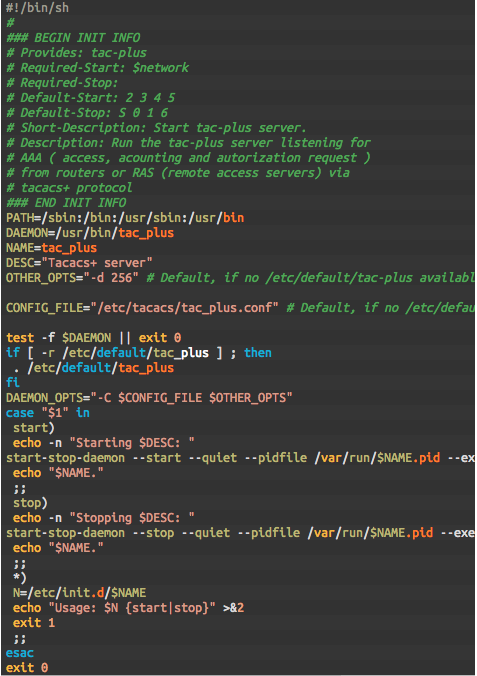
\includegraphics[scale=0.5]{img/tac_plus_script.png}
\caption{The start/stop script for tacacs}
\label{fig:}
\centering
\end{figure}
%</mtag22>

%<*mtag23>
\begin{figure}[H]
\centering
\captionsetup{width=.8\linewidth}
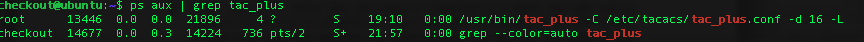
\includegraphics[scale=0.5]{img/ps_aux.png}
\caption{tac\_plus process}
\label{fig:}
\centering
\end{figure}
%</mtag23>

%<*mtag24>
\begin{figure}[H]
\centering
\captionsetup{width=.8\linewidth}
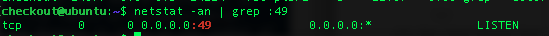
\includegraphics[scale=0.5]{img/netstat.png}
\caption{Tacacs listens on port 49}
\label{fig:}
\centering
\end{figure}
%</mtag24>

%<*mtag25>
\begin{figure}[H]
\centering
\captionsetup{width=.8\linewidth}
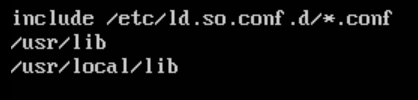
\includegraphics[scale=0.5]{img/ld_conf.png}
\caption{}
\label{fig:}
\centering
\end{figure}
%</mtag25>

%<*mtag26>
\begin{figure}[H]
\centering
\captionsetup{width=.8\linewidth}
\includegraphics[scale=0.5]{img/Ex1S0_1.png}
\caption{}
\label{fig:}
\centering
\end{figure}
%</mtag26>

%<*mtag27>
\begin{figure}[H]
\centering
\captionsetup{width=.8\linewidth}
\includegraphics[scale=0.5]{img/Ex1S0_1.png}
\caption{}
\label{fig:}
\centering
\end{figure}
%</mtag27>

%<*mtag28>
\begin{figure}[H]
\centering
\captionsetup{width=.8\linewidth}
\includegraphics[scale=0.5]{img/Ex1S0_1.png}
\caption{}
\label{fig:}
\centering
\end{figure}
%</mtag28>

%<*mtag29>
\begin{figure}[H]
\centering
\captionsetup{width=.8\linewidth}
\includegraphics[scale=0.5]{img/Ex1S0_1.png}
\caption{}
\label{fig:}
\centering
\end{figure}
%</mtag29>

%<*mtag30>
\begin{figure}[H]
\centering
\captionsetup{width=.8\linewidth}
\includegraphics[scale=0.5]{img/Ex1S0_1.png}
\caption{}
\label{fig:}
\centering
\end{figure}
%</mtag30>

%<*mtag31>
\begin{figure}[H]
\centering
\captionsetup{width=.8\linewidth}
\includegraphics[scale=0.5]{img/Ex1S0_1.png}
\caption{}
\label{fig:}
\centering
\end{figure}
%</mtag31>

%<*mtag32>
\begin{figure}[H]
\centering
\captionsetup{width=.8\linewidth}
\includegraphics[scale=0.5]{img/Ex1S0_1.png}
\caption{}
\label{fig:}
\centering
\end{figure}
%</mtag32>

%<*mtag33>
\begin{figure}[H]
\centering
\captionsetup{width=.8\linewidth}
\includegraphics[scale=0.5]{img/Ex1S0_1.png}
\caption{}
\label{fig:}
\centering
\end{figure}
%</mtag33>

%<*mtag34>
\begin{figure}[H]
\centering
\captionsetup{width=.8\linewidth}
\includegraphics[scale=0.5]{img/Ex1S0_1.png}
\caption{}
\label{fig:}
\centering
\end{figure}
%</mtag34>

%<*mtag35>
\begin{figure}[H]
\centering
\captionsetup{width=.8\linewidth}
\includegraphics[scale=0.5]{img/Ex1S0_1.png}
\caption{}
\label{fig:}
\centering
\end{figure}
%</mtag35>

%<*mtag36>
\begin{figure}[H]
\centering
\captionsetup{width=.8\linewidth}
\includegraphics[scale=0.5]{img/Ex1S0_1.png}
\caption{}
\label{fig:}
\centering
\end{figure}
%</mtag36>

%<*mtag37>
\begin{figure}[H]
\centering
\captionsetup{width=.8\linewidth}
\includegraphics[scale=0.5]{img/Ex1S0_1.png}
\caption{}
\label{fig:}
\centering
\end{figure}
%</mtag37>

%<*mtag1>
\begin{figure}[H]
\centering
\captionsetup{width=.8\linewidth}
\includegraphics[scale=0.5]{img/Ex1S0_1.png}
\caption{}
\label{fig:}
\centering
\end{figure}
%</mtag38>

%<*mtag39>
\begin{figure}[H]
\centering
\captionsetup{width=.8\linewidth}
\includegraphics[scale=0.5]{img/Ex1S0_1.png}
\caption{}
\label{fig:}
\centering
\end{figure}
%</mtag39>

%<*mtag40>
\begin{figure}[H]
\centering
\captionsetup{width=.8\linewidth}
\includegraphics[scale=0.5]{img/Ex1S0_1.png}
\caption{}
\label{fig:}
\centering
\end{figure}
%</mtag40>

%<*mtag42>
\begin{figure}[H]
\centering
\captionsetup{width=.8\linewidth}
\includegraphics[scale=0.5]{img/Ex1S0_1.png}
\caption{}
\label{fig:}
\centering
\end{figure}
%</mtag41>

%<*mtag43>
\begin{figure}[H]
\centering
\captionsetup{width=.8\linewidth}
\includegraphics[scale=0.5]{img/Ex1S0_1.png}
\caption{}
\label{fig:}
\centering
\end{figure}
%</mtag43>

%<*mtag44>
\begin{figure}[H]
\centering
\captionsetup{width=.8\linewidth}
\includegraphics[scale=0.5]{img/Ex1S0_1.png}
\caption{}
\label{fig:}
\centering
\end{figure}
%</mtag44>

%<*mtag45>
\begin{figure}[H]
\centering
\captionsetup{width=.8\linewidth}
\includegraphics[scale=0.5]{img/Ex1S0_1.png}
\caption{}
\label{fig:}
\centering
\end{figure}
%</mtag45>

%<*mtag46>
\begin{figure}[H]
\centering
\captionsetup{width=.8\linewidth}
\includegraphics[scale=0.5]{img/Ex1S0_1.png}
\caption{}
\label{fig:}
\centering
\end{figure}
%</mtag46>

%<*mtag47>
\begin{figure}[H]
\centering
\captionsetup{width=.8\linewidth}
\includegraphics[scale=0.5]{img/Ex1S0_1.png}
\caption{}
\label{fig:}
\centering
\end{figure}
%</mtag47>

%<*mtag48>
\begin{figure}[H]
\centering
\captionsetup{width=.8\linewidth}
\includegraphics[scale=0.5]{img/Ex1S0_1.png}
\caption{}
\label{fig:}
\centering
\end{figure}
%</mtag48>

%<*mtag49>
\begin{figure}[H]
\centering
\captionsetup{width=.8\linewidth}
\includegraphics[scale=0.5]{img/Ex1S0_1.png}
\caption{}
\label{fig:}
\centering
\end{figure}
%</mtag49>

%<*mtag50>
\begin{figure}[H]
\centering
\captionsetup{width=.8\linewidth}
\includegraphics[scale=0.5]{img/Ex1S0_1.png}
\caption{}
\label{fig:}
\centering
\end{figure}
%</mtag50>